% Just The Docs Front Matter
% title: Subglacial Hydrology of Helheim Glacier (SHAKTI)
% parent: Tutorials
% has_children: false
% has_toc: false

\subsection{Subglacial Hydrology of Helheim Glacier (SHAKTI)} \label{sec:using-issm-tutorials-helheimshakti}
\subsubsection{Goals}
\begin{itemize}
	\item Use SHAKTI model to simulate subglacial hydrology of Helheim Glacier in southeast Greenland
	\item Follow an example of how to set up a SHAKTI hydrology simulation on a real-world glacier
	\item Learn how to run a two-way coupled hydrology--velocity model with SHAKTI-ISSM
	\item Run a coupled SHAKTI-ISSM simulation of winter base-state hydrology
	\item Run a coupled SHAKTI-ISSM simulation with transient seasonal meltwater inputs (distributed and point inputs)
\end{itemize}

\subsubsection{Introduction}
In this example, the main goal is to set up a subglacial hydrology simulation using the SHAKTI model, coupled with ice velocity on a real Greenland outlet glacier. In order to build an operational simulation of Helheim Glacier as an example, we will follow these steps:
\begin{itemize}
	\item Load your Helheim Glacier model created in the `Modeling Helheim Glacier tutorial
	\item Set the hydrology model to SHAKTI and set up friction coupling
	\item Set SHAKTI-specific hydrology parameters
	\item Run a transient two-way coupled simulation with zero meltwater input to generate the winter base state drainage system
	\item Set up and run two-way coupled seasonal simulations with prescribed distributed meltwater input and point meltwater inputs
\end{itemize}

Files needed for this tutorial can be found in \lstinlinebg|<ISSM_DIR>/examples/HelheimSHAKTI/|. This tutorial begins from a model of Helheim Glacier generated in the 
%__@LATEX_ONLY_START@__
\hyperref[sec:using-issm-tutorials-helheim]{`Modeling Helheim Glacier' tutorial}.
%__@LATEX_ONLY_END@__
%__@MARKDOWN_ONLY_START@__
%<a href="helheim">'Modeling Helheim Glacier' tutorial</a>.
%__@MARKDOWN_ONLY_END@__

\subsubsection{Load model}
The first step in the \lstinlinebg|runme.m| file is to load the model of Helheim Glacier created in the previous tutorial. We turn off the inversion now.

\subsubsection{Set up SHAKTI subglacial hydrology model}
In the \lstinlinebg|runme.m| file, we set the hydrology model to SHAKTI:
\lstinlinebg|md.hydrology = hydrologyshakti();|

Next, we initialize the SHAKTI-specific hydrological parameters:
\begin{itemize}
	\item Distributed meltwater input ("englacial input") (m yr\textsuperscript{-1})
	\item Point meltwater input ("moulin input") (m\textsuperscript{3} s\textsuperscript{-1})
	\item Initial hydraulic head (m)
	\item Initial subglacial gap height (m)
	\item Typical bed bump height and spacing (m)
	\item Initial Reynolds number
	\item Boundary conditions (prescribed head for thin ice and ice-free elements)
\end{itemize}

\subsubsection{Define coupling and friction}
We turn on the coupling between SHAKTI and ISSM through \lstinlinebg|md.transient| and \lstinlinebg|md.friction.coupling|. This tutorial uses the Budd-type sliding law.

\begin{itemize}
	\item To turn on SHAKTI, set \lstinlinebg|md.transient.ishydrology = 1|.
	\item To solve for stress balance in the transient simulation, set \lstinlinebg|md.transient.isstressbalance = 1| and \lstinlinebg|md.friction.coupling = 4|.
	\item To run stand-alone SHAKTI without evolving velocity, set \lstinlinebg|md.transient.isstressbalance = 0|.
\end{itemize}

\subsubsection{Run a winter simulation}
The final step before running is to define the time step and final time of the simulation. Note that the time step and final time set in years, so make sure to convert appropriately. Small time steps on the order of 1 hour are typically functional for SHAKTI, but feel free to experiment with this.

The model will take a while to run, exactly how long will vary depending on your final time, time step, how many processors you are using, and mesh resolution. If you are running a long simulation, you might not want to save model output at every time step and can reduce the output file size through \lstinlinebg|md.settings.output_frequency| (for example, with a time step of 1 hour, you would set \lstinlinebg|md.settings.output_frequency = 24;| to save output once every day).

The model you have set up currently specifies zero meltwater inputs (\lstinlinebg|md.hydrology.englacial_input| and \lstinlinebg|md.hydrology.moulin_inputs| are both zero everywhere). This represents winter conditions, when all water at the bed is generated via basal melt by geothermal flux, frictional heat from sliding, and turbulent dissipation.

You can examine the output spatially by plotting different quantities. For example, here are plots of velocity, effective pressure, basal water flux, and hydraulic head after 30 days:
\begin{lstlisting}
plotmodel(md, 'data', md.results.TransientSolution(end).Vel, 'title', 'Velocity (m/yr', ...
	'data', md.results.TransientSolution(end).EffectivePressure, 'title', 'Effective Pressure (Pa)')
\end{lstlisting}
\begin{figure}[h!]
	\begin{center}
	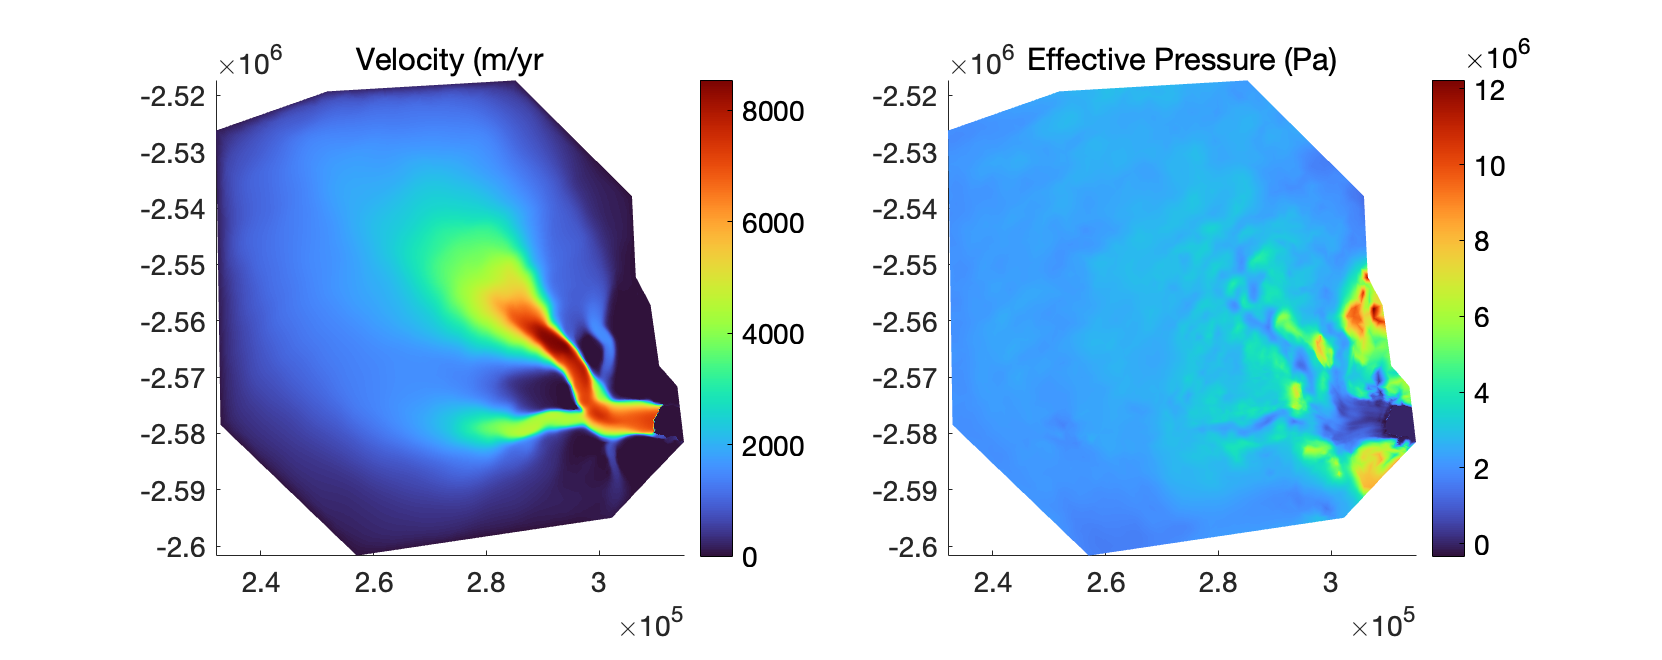
\includegraphics[width=\textwidth]{\assetsParentPath/assets/img/using-issm/tutorials/helheimshakti/figure_vel_N.png}
	\end{center}
\end{figure}

\begin{lstlisting}
plotmodel(md, 'data', log10(md.results.TransientSolution(end).HydrologyBasalFlux, 'title', 'log_{10}(Basal Water Flux) (m^2 s^{-1})', ...
	'data', md.results.TransientSolution(end).HydrologyHead, 'title', 'Head (m)')
\end{lstlisting}
\begin{figure}[h!]
	\begin{center}
	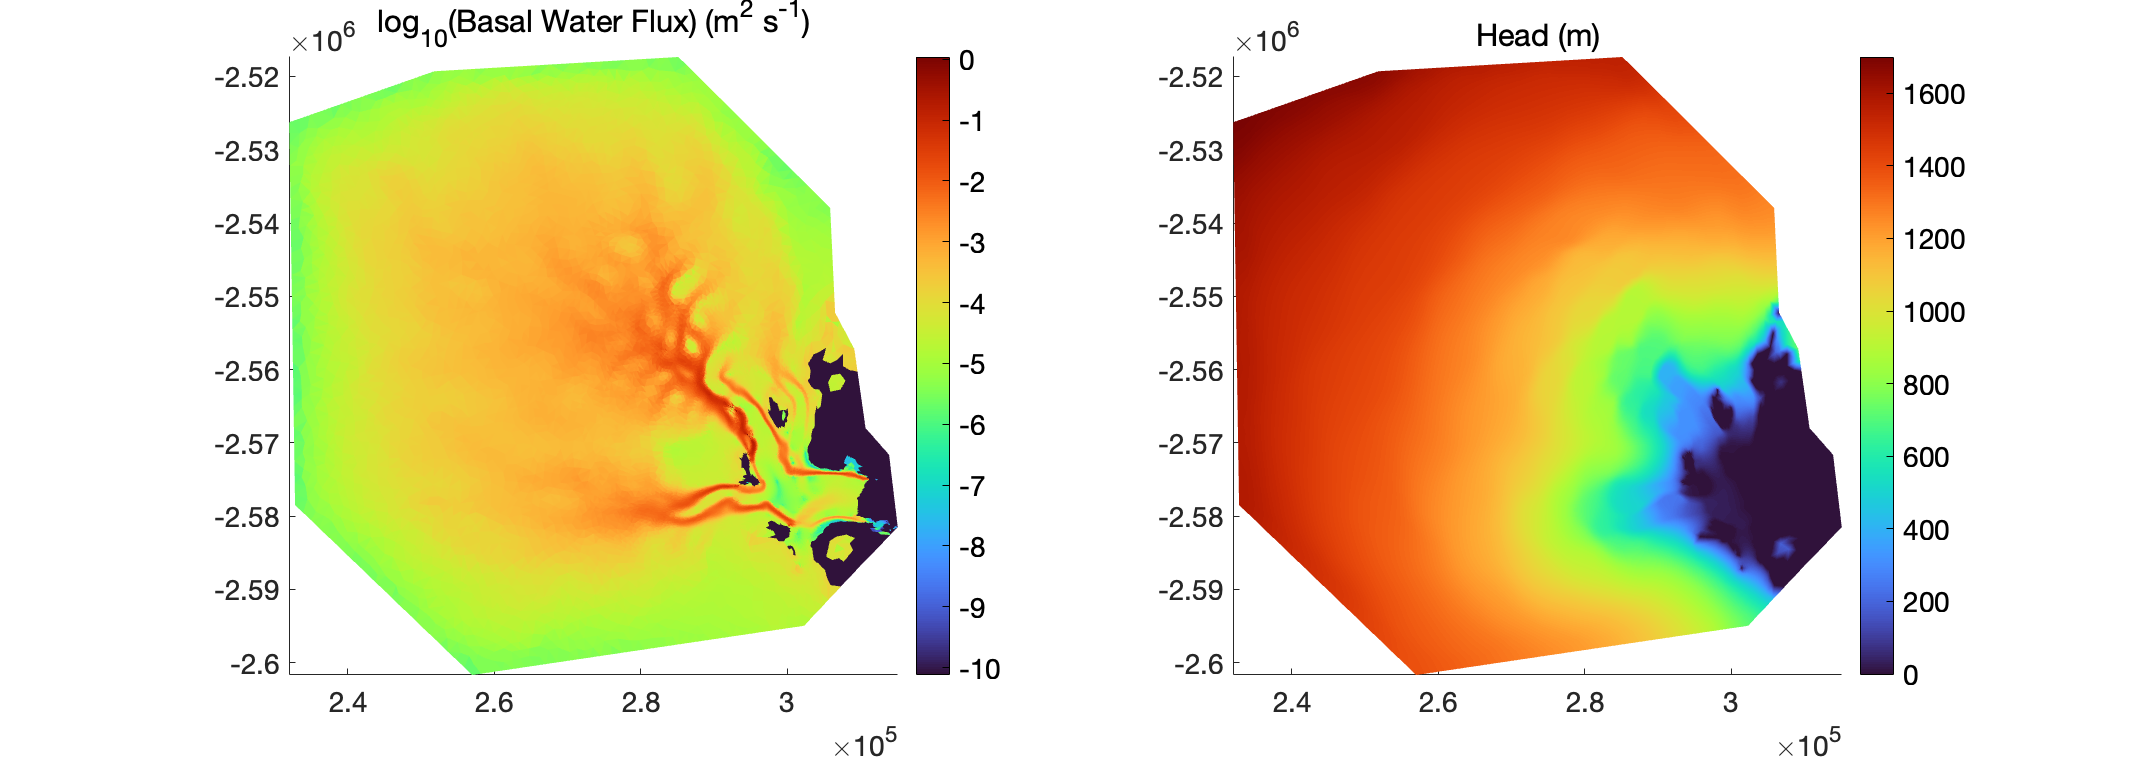
\includegraphics[width=\textwidth]{\assetsParentPath/assets/img/using-issm/tutorials/helheimshakti/figure_q_h.png}
	\end{center}
\end{figure}

If you are interested in a steady state, check convergence to a steady winter state by comparing \lstinlinebg|md.results.TransientSolution(end).Vel| and \lstinlinebg|md.results.TransientSolution(end).EffectivePressure| with the previous time step. You will probably need to run for a year or two for the system to fully equilibrate.

\subsubsection{Continuing a simulation}
You may find it helpful to continue a simulation from the end state of a previous simulation. This can be useful for running long simulations in segments or exploring different forcing from a common initialized state. Use the script below to continue a previous simulation, which sets the relevant initial parameters accordingly:

\begin{lstlisting}
% runme script to continue a coupled SHAKTI-ISSM simulation, continuing from
% end state of a previous simulation

clear all; close all

% Load the model you want to begin from
load Models/your_shaktiissm_model_name.mat

% Starting conditions from end of previous simulation
md.hydrology.head = md.results.TransientSolution(end).HydrologyHead;
md.hydrology.gap_height = md.results.TransientSolution(end).HydrologyGapHeight;
md.hydrology.reynolds = md.results.TransientSolution(end).HydrologyBasalFlux ./ 1.787e-6;
md.hydrology.reynolds(md.hydrology.reynolds == 0) = 1;

md.initialization.vx = md.results.TransientSolution(end).Vx;
md.initialization.vy = md.results.TransientSolution(end).Vy;
md.initialization.vel = md.results.TransientSolution(end).Vel;

% Time-stepping
md.timestepping.time_step = 3600 / md.constants.yts; % Time step (in years)
md.timestepping.final_time = 365 / 365;
md.settings.output_frequency = 24;

md.cluster = generic('np', 8);
md.verbose.solution = 1;
md = solve(md, 'Transient');
\end{lstlisting}

\subsubsection{Seasonal meltwater inputs}
Meltwater inputs can be added through two options:
\begin{itemize}
	\item Distributed meltwater input (e.g. for highly crevassed regions): \lstinlinebg|md.hydrology.englacial_input| (units of m yr\textsuperscript{-1})
	\item Point inputs to represent discrete crevasses or moulins: \lstinlinebg|md.hydrology.moulin_input| (units of m\textsuperscript{3} s\textsuperscript{-1})
\end{itemize}

Both types of meltwater input are spatially variable and can be prescribed as either constant in time (\lstinlinebg|size(md.mesh.numberofvertices, 1)|) or time-varying (\lstinlinebg|size(md.mesh.numberofvertices + 1, length(timevec))|). The sample code below includes example syntax for setting these meltwater inputs. Get creative and experiment with different combinations!
\begin{lstlisting}
% Time-stepping
md.timestepping.time_step = 3600 / md.constants.yts; % Time step (in years)
md.timestepping.final_time = 365 / 365;
timevec = 0:md.timestepping.time_step:md.timestepping.final_time;
md.settings.output_frequency = 24;

% To prescribe distributed meltwater inputs:
% Steady distributed meltwater inputs:
md.hydrology.englacial_input = zeros(md.mesh.numberofvertices, 1);
md.hydrology.englacial_input(:) = **set values here, can vary spatially**;

% Time-varying distributed meltwater inputs:
% Initialize the matrix as zeros
md.hydrology.englacial_input = zeros(md.mesh.numberofvertices + 1, length(timevec));
% Set the final column to be a time index
md.hydrology.englacial_input(end, :) = timevec;
% Example: low-elevation distributed meltwater inputs
le = find(md.geometry.surface <= 900); % Find low-elevation vertices below 900 m
for nv=1:length(le)
md.hydrology.englacial_input(le(nv), :) = <<your data or function here>>;
end

% To prescribe point meltwater inputs:
% Example: Steady input into firn aquifer crevasse drainage points
% Find high-elevation crevasse input points from firn aquifer at 1500 m
he = find(md.geometry.surface >= 1500 & md.geometry.surface <= 1515);
highieb = 1.5855 / size(he, 1); % Use 50e6 m^3/yr, converted to m^3/s, divided evenly between eligible points
md.hydrology.moulin_input = zeros(md.mesh.numberofvertices, 1);
md.hydrology.moulin_input(he) = highieb;

% For time-varying point inputs:
md.hydrology.moulin_input = zeros(md.mesh.numberofvertices + 1, length(timevec));
md.hydrology.moulin_input(end, :) = timevec;
md.hydrology.moulin_input(1:end-1, :) = **set values here, can vary spatially and temporally**
\end{lstlisting}

\subsubsection{Resources}
For more details about the SHAKTI model and applications to Helheim Glacier, please see the
following references: \cite{Sommers2018,Sommers2023,Sommers2024}.

\clearpage % Make sure all figures are placed before next section
